\section{tree\_pureness} \label{sec-pureness}

\subsection{General}

\emph{tree\_pureness} is a tool that can compare a Tree and the layer wise
cluster separations generated by an adaptive clustering run with the tools
outlined in section \ref{sec-adaptive-clust} with a ground trouth set.
Ground trouth sets can for instance be generated using the
\emph{split\_set\_from\_annotation} (c.f. section
\ref{sec-ssannotation}) or \emph{split\_set\_from\_swarm}
(c.f. \ref{sec-ssannotation})
tool if a comparison agains such tools is the reason for using this
utility. \emph{Tree\_purness} calculates three indicies:
\begin{enumerate}
\item Pureness Index,
\item Cluster correspondance,
  and
\item Impure over pure.
\end{enumerate}
This tool as the major tree quality measurement tool if a ground truth
for a tree is known. 

\subsection{Usage}
The tool can be called like
\lstset{language=bash,
  caption={Calling the \emph{tree\_pureness} tool},
  label=lst-treepureness-call}
\begin{lstlisting}
tree_pureness [fasta] [ground-truth] [split-sets] > [output]
\end{lstlisting}
with the following arguments:
\begin{enumerate}
\item \emph{fasta} A FASTA dataset of sequences that a tree has been
  built from, and that a ground truth clustering set is known from.
\item \emph{ground-truth} A binary \emph{split-set} file that contains
  the clustering of the groud truth.
\item \emph{split-sets} The resulting split sets from an adaptive
  clustering run, that represent a full tree.
\item \emph{output} Output is a text file containing each layer in a
  tree the three indices that allow for a comparison to ground truth.
\end{enumerate}

\subsection{Algorithm}
The program defines the three indices:
\begin{enumerate}
\item \emph{Pureness:} We define the Pureness Index to be:
  \begin{equation}
    P_{l} =
    \frac{1}{n_{l,\mathrm{inp}}}
    \sum_{i=1}^{n_{l,\mathrm{inp}}}\sum_{k=1}^{n_{\mathrm{target}}}
    \frac{f_{l,i,k}^{<50\%}}{C_{l,i}},
    \label{eqn-pureness}
  \end{equation}
  where $l$ represents the layer of a tree, $n_{l,\mathrm{inp}}$ the
  number of inpure clusters, hence the clusters that are mixture of
  two partitions from the inital truth dataset to compare to,
  $n_{\mathrm{target}}$ the number of partitions in the original
  truth dataset, $f_{l,i,k}^{<50\%}$ the number of elements
  belonging to partition $k$ of the truth dataset in the inpure
  cluster indexed by $i$ in layer $l$ if this number represents less
  then 50\% of the elements in the inpure cluster otherwise
  $f_{l,i,k}^{<50\%}$ represents the total number of elements in the
  inpure cluster minus the elements in this cluster that belong to
  the partion of the truth dataset that is indexed by $k$. Finally
  $C_{l,i}$ represents the total number of elements in the inpure
  cluster in layer $l$ indexed by $i$.
\item \emph{Cluster correspondance}: It is straight forward to
  reason that pureness as define above is not enough, as a
  partitioning with enough small clusters would yield highly pure
  clusters but not a meaningfull partioning, as such we further
  define:
  \begin{equation}
    S_{l}=\frac{|n_{l}-n_{\mathrm{target}}|}{n_{\mathrm{target}}}, \label{eqn-c-corr}
  \end{equation}
  where $n_{l}$ is the number of clusters in layer $l$ to be the
  measure of correspondance between the number of clusters in the
  truth partioning and the number of clusters obtained in our
  partitioning.
\item \emph{Impureness over pureness}: Finally we argue that we need a
  third value in order to describe the quality of our tree:
  \begin{equation}
    I_{l}=\frac{n_{l,\mathrm{inp}}}{n_{l}}. \label{eqn-impure-pure}
  \end{equation}
  $I_{l}$ represents the number of inpure clusters, hence those who
  contain mixtures of partitions from the truth partitioning over
  the number of clusters that are pure.
\end{enumerate}
An exmaple of clustering and the calculation of the three indices is shown
in figure \ref{fig-pureness}.
\begin{figure}
  \begin{center}
  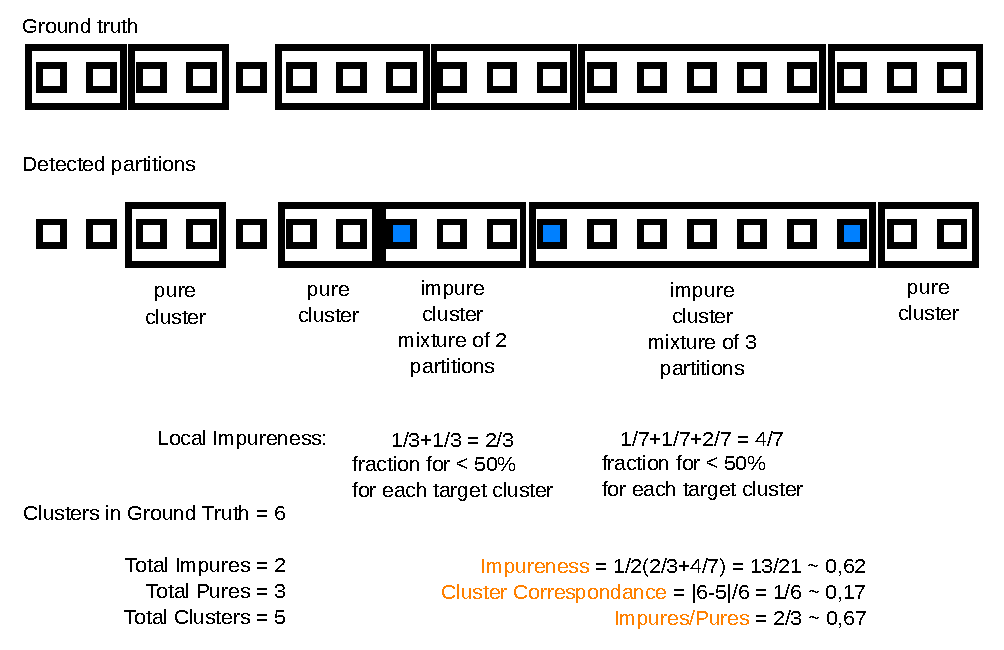
\includegraphics[scale=0.9]{pureness.pdf}
  \caption{A groud truth and a computed clustering. The figure shows how
    the cluster indices: Pureness, Cluster Correspondance and
    Impureness over Pureness are calculated.}
  \label{fig-pureness}
  \end{center}
\end{figure}

\subsection{Example}
We call \emph{tree\_purness} like
\lstset{language=bash,
  caption={Example of the \emph{tree\_pureness} tool},
  label=lst-treepureness-example}
\begin{lstlisting}
tree_purness test.fasta ground-truth /tmp/s* > /tmp/pureness
\end{lstlisting}
where \emph{test.fasta} is a dataset and \emph{ground-truth} is a
a binary \emph{split-set} describing the clustering we care comparing
all the clusterings in the tree to. \emph{/tmp/s*} is the wildcard to
select all the binary clusterings that have been produced for a
complete tree using an adaptive clustering run (c.f. section
\ref{sec-adaptive-clust}).
A resulting \emph{/tmp/pureness} then might look like this:
\lstset{language={},
  caption={Example output of the \emph{tree\_pureness} tool},
  label=lst-treepureness-output}
\begin{lstlisting}
0.207187        1.015385        0.259542
0.207658        0.761538        0.288210
0.214303        0.407692        0.267760
0.267122        0.230769        0.281250
0.270319        0.007692        0.297710
0.278394        0.176923        0.280374
0.333774        0.330769        0.264368
0.301733        0.415385        0.315789
0.327885        0.569231        0.267857
\end{lstlisting}
with three tablator seperated values per line, where the first value
is the Pureness, the scond the Cluster Correspondance and the third
the Impureness over Pureness value. Using \emph{gnuplot} for instance
one can create a three value diagram in order to judge if a level of
the tree yields the accuracy requested to the ground truth. Such an
example is shown in figure \ref{fig-pureness-example}.
\begin{figure}
  \begin{center}
    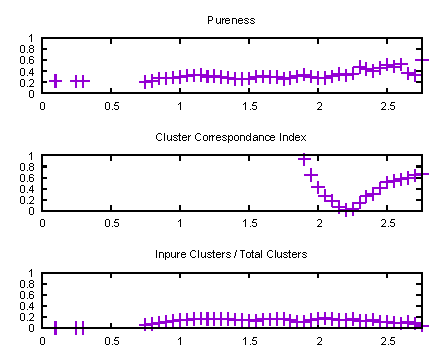
\includegraphics[scale=1.4]{pureness-example.pdf}
    \caption{An example of a visual representation of the data
      obtained from the \emph{tree\_pureness} tool. On the abscissa
      the $\epsilon$ value is shown, which resides in the output of
      the adaptive clustering run for each
      value. (c.f. section \ref{sec-adaptive-clust}).}
    \label{fig-pureness-example}
  \end{center}
\end{figure}

\subsection{Implementation}
The interface is implemented in \emph{tree\_purness.c}. The
functionality is to be found in \emph{cluster\_io.c}. 

